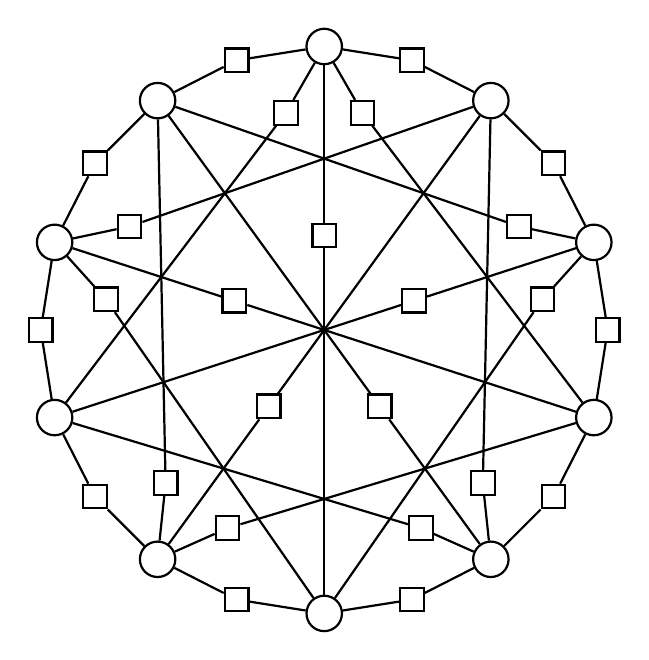
\begin{tikzpicture}[thick,scale=0.8]
%\node[circle,draw=black,label={}] (v1) at (-4,0){};
%\node[shape=rectangle,draw=black,label={}] (c1) at (-2,0){\color{red}{0}};
%\path [-,thick] (v1) edge node[left] {} (c1); 
%\draw[->,violet,thick]  (-2.3,-0.2) to node[left]{\hspace{-.35 in}0}(-3,-0.2);


% Draw the nodes in polar coordinates

%%%%%%%%%%%%%%%%%%%% Outer Cycle %%%%%%%%%%%%%%%%%%%%%%%%%%
%variable nodes
\foreach \index in {1, ..., 9, 10}
{
    \node[circle, draw=black, minimum size=4.5mm] (v\index) at ({-((\index-1)*36)+90}:4.5) {};
}

\foreach \index in {1, ..., 9, 10}
{
    \node[shape=rectangle, draw=black, minimum size=3mm] (c\index) at ({-((\index-1)*36+18)+90}:4.5) {};
}

%Draw outer cycle
\foreach \index in {1, ..., 9, 10}
{
    \path [-,thick] (v\index) edge node[left] {} (c\index);  
}
\foreach \index in {1, 2, ..., 9}
{
    \path [-,thick] (c\index) edge node[left] {} (v\the\numexpr\index+1\relax);  
}
\path [-,thick] (c10) edge node[left] {} (v1);  

%%%%%%%%%%%%%%%%%%%% 2nd Cycle %%%%%%%%%%%%%%%%%%%%%%%%%%
\foreach \index in {0,1,..., 4}
{
    \node[shape=rectangle, draw=black, minimum size=3mm] (c\the\numexpr\index*2+11\relax) at ({100-72*\index}:3.5) {};
    \node[shape=rectangle, draw=black, minimum size=3mm] (c\the\numexpr\index*2+12\relax) at ({80-72*\index}:3.5) {};
}
\foreach \index in {1,3,5,7,9}
{
    \path [-,thick] (v\index) edge node[left] {} (c\the\numexpr\index+10\relax);
    \path [-,thick] (v\index) edge node[left] {} (c\the\numexpr\index+11\relax);  
}
\path [-,thick] (v8) edge node[left] {} (c11);
\path [-,thick] (v8) edge node[left] {} (c16);
\path [-,thick] (v4) edge node[left] {} (c12);
\path [-,thick] (v4) edge node[left] {} (c17);
\path [-,thick] (v10) edge node[left] {} (c13);
\path [-,thick] (v10) edge node[left] {} (c18);
\path [-,thick] (v6) edge node[left] {} (c14);
\path [-,thick] (v6) edge node[left] {} (c19);
\path [-,thick] (v2) edge node[left] {} (c15);
\path [-,thick] (v2) edge node[left] {} (c20);

%%%%%%%%%%%%%%%%%%%% 3rd Cycle %%%%%%%%%%%%%%%%%%%%%%%%%%
\foreach \index in {0,1,..., 4}
{
    \node[shape=rectangle, draw=black, minimum size=3mm] (c\the\numexpr\index+21\relax) at ({90-72*\index}:1.5) {};
}
\path [-,thick] (c21) edge node[left] {} (v1);
\path [-,thick] (c21) edge node[left] {} (v6);
\path [-,thick] (c22) edge node[left] {} (v3);
\path [-,thick] (c22) edge node[left] {} (v8);
\path [-,thick] (c23) edge node[left] {} (v5);
\path [-,thick] (c23) edge node[left] {} (v10);
\path [-,thick] (c24) edge node[left] {} (v2);
\path [-,thick] (c24) edge node[left] {} (v7);
\path [-,thick] (c25) edge node[left] {} (v4);
\path [-,thick] (c25) edge node[left] {} (v9);

\end{tikzpicture}